\def\bagrutTocEntry{\phantomsection\addcontentsline{toc}{subsection}{\texorpdfstring{سؤال $12$ امتحان $\mathrm{899271B}$ سنة $2025$}{سؤال 12 امتحان 899271B سنة 2025}}\global\let\bagrutTocEntry\relax}%
\includepdf[pages=-,pagecommand={\thispagestyle{empty}\bagrutTocEntry}]{../../../bagrut_questions/oop/oop_2025_899271B_12.pdf}


\ifwithsols
\begin{boxSolution}[\texorpdfstring{سؤال $12$ امتحان $\mathrm{899271B}$ سنة $2025$ - فرع أ}{سؤال 12 امتحان 899271B سنة 2025 - فرع أ}]
\textbf{أ.} الكائنات التي تكوّنت في \textenglish{Main} (علماً أنّ \textenglish{One.num = 18}):
\begin{center}
\begin{english}
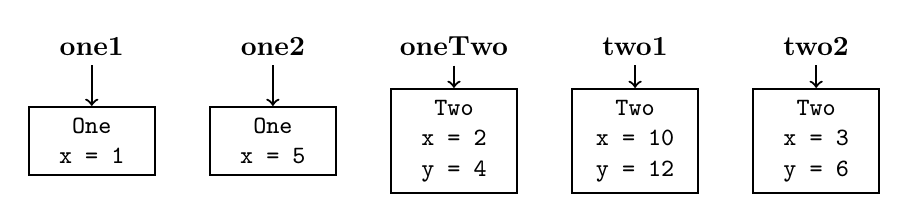
\begin{tikzpicture}[
    obj/.style={rectangle, draw, thick, align=center, font=\ttfamily\small, minimum width=1.6cm, inner sep=4pt}
]
    \node (v1) at (0, 1.2) {\textbf{one1}};
    \node[obj] (o1) at (0, 0) {\textbf{One}\\x = 1};
    \draw[->, thick] (v1) -- (o1);

    \node (v2) at (2.3, 1.2) {\textbf{one2}};
    \node[obj] (o2) at (2.3, 0) {\textbf{One}\\x = 5};
    \draw[->, thick] (v2) -- (o2);

    \node (v3) at (4.6, 1.2) {\textbf{oneTwo}};
    \node[obj] (o3) at (4.6, 0) {\textbf{Two}\\x = 2\\y = 4};
    \draw[->, thick] (v3) -- (o3);

    \node (v4) at (6.9, 1.2) {\textbf{two1}};
    \node[obj] (o4) at (6.9, 0) {\textbf{Two}\\x = 10\\y = 12};
    \draw[->, thick] (v4) -- (o4);

    \node (v5) at (9.2, 1.2) {\textbf{two2}};
    \node[obj] (o5) at (9.2, 0) {\textbf{Two}\\x = 3\\y = 6};
    \draw[->, thick] (v5) -- (o5);
\end{tikzpicture}
\end{english}
\end{center}

مُخرج العملية \textenglish{Main}:
\begin{boxCode}
\begin{english}
\begin{minted}{text}
One 1
One 2
One 1
Second
One 1
One 1
Second
\end{minted}
\end{english}
\end{boxCode}
\end{boxSolution}

\filbreak

\begin{boxSolution}[\texorpdfstring{سؤال $12$ امتحان $\mathrm{899271B}$ سنة $2025$ - فرع ب}{سؤال 12 امتحان 899271B سنة 2025 - فرع ب}]
\textbf{ب.} فحص الأوامر $1$–$10$:
\begin{enumerate}[label=\textbf{\arabic*.}, itemsep=0.3em]
    \item \textbf{سليم.} المُخرج: \textenglish{Total = 18}
    \item \textbf{سليم.} المُخرج: \textenglish{Total = 18}
    \item \textbf{سليم.} المُخرج: \textenglish{Mul = 1}
    \item \textbf{غير سليم (خطأ ترجمة).} النمط الساكن لـ \textenglish{oneTwo} هو \textenglish{One}، ولا توجد في \textenglish{One} عملية \textenglish{Mul()} بدون معطيات.
    \item \textbf{سليم.} المُخرج: \textenglish{Mul = 120}
    \item \textbf{سليم.} تستدعي \textenglish{One.Add} ($x = 1 + 2 = 3$). المُخرج: \textenglish{x = 3}
    \item \textbf{سليم.} تستدعي \textenglish{Two.Add} ($y = 12 + 4 = 16$). المُخرج: \textenglish{y = 16}
    \item \textbf{غير سليم (خطأ في زمن التشغيل).} الكائن الفعلي لـ \textenglish{one1} هو من نمط \textenglish{One} وليس \textenglish{Two}، لذا يفشل التحويل لأسفل \textenglish{(Two)one1}.
    \item \textbf{غير سليم (خطأ ترجمة).} لا يمكن جعل مؤشر من نمط الابن \textenglish{Two} يشير إلى كائن من نمط الأب \textenglish{One}.
    \item \textbf{سليم.} تستدعي \textenglish{One.Mul(1)} (تعيد $10$)، ولكن لا يُطبع شيء لعدم وجود أمر طباعة.
\end{enumerate}
\end{boxSolution}
\fi
\filbreak
